\documentclass[tikz]{standalone}

\begin{document}

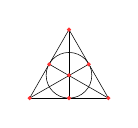
\begin{tikzpicture}
%%% LINES
    \draw[very thin] (0,0) -- (1,0);
    \draw[very thin] (0.5,0.87) -- (1,0);
    \draw[very thin] (0,0) -- (0.5,0.87);
    \draw[very thin] (0.5,0) -- (0.5,0.87);
    \draw[very thin] (1,0) -- (0.25,0.43);
    \draw[very thin] (0,0) -- (0.75,0.43);
    \draw[very thin] (0.5,0.29) circle (0.29);
%%% POINTS
    \filldraw[red!80] (0,0) circle (0.5pt);
    \filldraw[red!80] (0.5,0) circle (0.5pt);
    \filldraw[red!80] (1,0) circle (0.5pt);
    \filldraw[red!80] (0.75,0.43) circle (0.5pt);
    \filldraw[red!80] (0.5,0.87) circle (0.5pt);
    \filldraw[red!80] (0.25,0.43) circle (0.5pt);
    \filldraw[red!80] (0.5,0.29) circle (0.5pt);
\end{tikzpicture}

\end{document}